\documentclass[10pt,a4paper]{article}
\usepackage[latin1]{inputenc}
\usepackage{amsmath}
\usepackage{amsfonts}
\usepackage{amssymb}
\usepackage{graphicx}
\usepackage{eurosym}

\author{Group 16}
\title{Titan Expedition\\ Project 1.2 - Report}
\usepackage{titlesec}

%No idea about how this works, it is used to have numbered paragraphs
\setcounter{secnumdepth}{4}
\setcounter{tocdepth}{4}
\titleformat{\paragraph}
{\normalfont\normalsize\bfseries}{\theparagraph}{1em}{}
\titlespacing*{\paragraph}
{0pt}{3.25ex plus 1ex minus .2ex}{1.5ex plus .2ex}

\begin{document}
	\begin{titlepage}    
		\begin{center}    
			{\LARGE Maastricht University}\\
			\vspace{15pt}
			{\large Department of Data Science and Knowledge Engineering}
			\vspace{30pt}
			
			\hrule
			\vspace{15pt}
			{\Large Titan Expedition}\\
			\vspace{15pt}
			{\large Project 1-2 - Report}
			\vspace{15pt}
			\hrule
			
			\vspace{30pt}
			Group 16\\
			\vspace{15pt}
			
			\textit{Authors:}\\
			Jan-Felix De Man (i6201411)\\
			Selim Gilon (i6192074)\\
			Gyumin Oh (i6185378)\\
			Pietro Piccini (i6188338)\\
			Gianluca Vico (i6183186\\            
			\vspace{15pt}
			
			\textit{Supervisors:}\\
			Enrique Hortal Quesada\\
			\vspace{15pt}
			
			\textit{Examiners:}\\
			Siamak Mehrkanoon\\
			Nico Roos\\
			\vspace{15pt}
			
			\vspace*{\fill}
			Block 1.6\\
			Bouillonstraat 8-10, 6211 LH Maastricht, Netherlands\\
			26th July 2019
		\end{center}
	\end{titlepage}
	
	\newpage
	\section*{Preface}
	This report is a description of an approach to reach Saturn's hazy moon Titan, land on it and travel back to Earth with a realistic spaceship. It is intended for every scientific, mathematician, computer scientist or whoever is interested in the space's expeditions. This moon has never been reached by any astronaut in the history; only one probe has been sent to explore Saturn's largest moon. This spacecraft called "Huygens" \footnote{Rincon, P. (2005). BBC NEWS | Science/Nature | Huygens sends first Titan images. Retrieved from http://news.bbc.co.uk/2/hi/science/nature/4175099.stm} (part of the Cassini Mission) landed on in 2005. This is still the most distant landing of any human-made craft. The  Scientists agree that this celestial body is the most important place where to search for extraterrestrial life \footnote{Bortman, H. (2010). Life Without Water And The Habitable Zone. Retrieved from http://www.spacedaily.com/reports/Life\_Without\_Water\_And\_The\_Habitable\_Zone\_999.html}. Nasa's scientists are actually working on a mission called "Dragonfly" \footnote{Bartels, M. (2019). NASA May Decide This Year to Land a Drone on Saturn's Moon Titan. Retrieved from https://www.space.com/43010-dragonfly-mission-would-put-a-drone-on-titan.html} to go again there. In this report, you will discover a way that the team made to try to explore this unknown moon.
	
	\section*{Abstract}
	The purpose of this project is to bring a manned mission to land safely on Titan and return back to Earth. Some other goals have to be reached such as making the travel as cheap as possible by computing the best trajectory using orbits and also making the duration of the trip as short as possible. The plan is to use as many realistic and correct data as possible and keep a pretty high accuracy in all the calculations. \\
	A lot of research about the different parts of the problem is required, so Nasa's data, for example, have been a really important source to get a deeper comprehension and decomposition of this big problem. The knowledge from the course "Numerical Mathematics" has also been very helpful to solve many equations in this program. After several versions and improvements, the program is now able to calculate the correct trajectory, land on Titan and come back to Earth. \\
	This reports aims to become a source for further improvements in this field.
	
	\newpage
	
	\tableofcontents
	\newpage
	
	%%%%%%%%%%%%%%%%%%%%%%%%%
	\section{List}
	\subsection{Abbreviations}
	\begin{itemize}
		\item $\vec{a}$: acceleration vector
		\item $a$: acceleration value
		\item $\vec{F}$: vector
		\item $G$: gravitational constant
		\item $h$: step size
		\item $I$: inertia momentum
		\item $\vec{L}$: angular momentum
		\item $m$: mass
		\item $\vec{\omega}$: angular velocity
		\item $\|\vec{r}\|$: 2-norm of $\vec{r}$
		\item $\vec{\tau}$: torque momentum
		\item $\vec{v}$: velocity vector
		\item $v$: velocity value        
		\item $w_i$: approximation of $y$ at the $i$-th iteration
		\item $\dot{y}(t)$: derivative of $y(t)$    
		\item Spaceship, rocket, shuttle and probe are used as synonyms     
	\end{itemize}
	\subsection{Tables}
	\begin{itemize}
		\item Table 1: Landing
		\item Table 2: Rotation influence
		\item Table 3: Initial velocity
		\item Table 4: Wind strength
		\item Table 5: Error analysis
	\end{itemize}
	
	\subsection{Figures}
	\begin{itemize}
		\item Figure 1: Catapult launcher
		\item Figure 2: Trajectory algorithm flowchart     
		\item Figure 3: Adams-Bashforth's relative error compared to Euler's
		\item Figure 4: Wind model
	\end{itemize}
	
	%%%%%%%%%%%%%%%%%%%%%%%%%%
	\section{Project description}
	
	\subsection{Introduction}
	Space travel and exploration has been on human's minds for as long as they have grasped the idea of "outer space". For ages, people dreamt of heading up to the moon and to fly between the stars. As mankind developed and was able to fully explore the planet Earth, the urge to explore the rest of the universe increased. It was not until recently that this became more than a dream. In 1961, Yuri Gagarin, the first living person to return from a space mission, completed the first orbit around Earth. A new era of (human) space exploration had started!\\
	
	A total of 12 men have landed on the moon and lived to tell the story. Mankind now launches more than 100 rockets into space per year. Everything seems possible for the extra-terrestrial explorers!\\
	
	This report is meant for everyone who would like to know more about a complete, safe space trip and its simulation. It is rather an introduction to this topic and its digital implementation. \\
	
	\subsection{Background}
	There are 62 moons orbiting around Saturn, the twentieth-most distant of these is called Titan. This moon is larger than Mercury, which makes it the second-largest moon in our Solar System, only topped by Jupiter's Ganymede. It was discovered in 1655 by the Dutch astronomer Christiaan Huygens, after whom the space Cassini-Huygens space mission was named. Titan is the only moon in our Solar System with a dense atmosphere, which was previously mistaken for a bigger size until the previously mentioned space mission. The biggest shock this mission revealed, however, was the discovery of liquid hydrocarbon lakes in its polar regions. Its atmosphere consists mostly of nitrogen. This creates ethane and methane clouds, which results in Earth-like weather. Titan has its own climate, which results in the making of dunes, rivers, lakes and seas. Although not made from water, this moon looks a lot like the place mankind calls home. 
	
	\subsection{Problem description}
	
	The objective of this project is to simulate our Solar System, in that simulation: launch a rocket to Titan, land it safely on its surface and bring it back to Earth. 
	In order to start tackling this problem, a physically correct simulation of the Solar System is needed. Using this model probes are launched from Earth. These probes behaves like cannonballs, launched from a cannon on Earth's surface. These so called exploratory missions help explore the workings of the physical simulation of the Solar System, which is based on gravity, and to develop an algorithm to calculate the trajectory of the probe. Once we have hit Titan with one of the probes, we know with which velocity to launch it at what point in time and are thus able to reach Saturn's moon.\\    
	
	Landing a rocket safely is a difficult mission. In order to land a rocket on a planet, it has to orbit the planet first. Once this is done, it has to align its direction so it can enter the orbit. In this phase of the landing the rocket is influenced by atmospheric factors, such as the wind. it needs to stabilize the rotation the wind inflicts, as the rocket can land straight and safe. The controllers of the rocket tries to keep the optimal alignment and to land with a minimum velocity, because obviously it is unsafe to land with a high speed.\\
	
	In this phase of the mission, the rocket is launched from Titan towards mother Earth. Assuming that there is a launching station on Titan, we follow the same approach as we did on Earth: launch the rocket with a given velocity. Then the rocket, following the optimal trajectory, returns eventually to the Earth. To optimize the fuel usage, we chose the launching method, instead of letting the engines steer the rocket all the way back.
	
	
	\subsection{Research questions}
	The objective of this research is to understand how to launch a spaceship from Earth to another celestial body and how to calculate its trajectory. Then it studies how to land the spaceship safely, even in extreme wind conditions, and how to come back. Furthermore it is investigated how to optimize fuel usage and how to minimize the overall costs.
	
	
	
	\subsection{Report structure}
	Chapter 3 starts with some explanations about the physics and the equation solvers of the Solar System. The rest of this section is a detailed description of the spaceship. Chapter 4 is reserved to the launching methods from the different planets. It also includes the algorithm's details for the trajectory. All the optimizations made during this project can be found in Chapter 6. The chapter 7 is following with different instructions about the graphical user interface and its insights. The next Chapter contains the experiments' details. The results of these are in Chapter 9. The last one lists conclusions from the whole experiment. It also mentions the improvements that the team would like to do in the future.
	
	
	%%%%%%%%%%%%%%%%%%%%%%%%%    
	\section{Models}
	
	\subsection{Solar System}
	\subsubsection{Physical approach and alternatives}
	To digitally simulate the Solar System, Newton's gravitational law is used. The model is based on the equation $\vec{F} = \frac{\vec{r}}{|\vec{r}|} G \dfrac{m_1 m_2}{|\vec{r}|^2} $. This means that the gravitational force F is equal to the product of the masses of both objects, divided by the distance squared, multiplied by the gravitational constant G. Or in other words: the bigger the mass and the closer the distance is, the bigger the force is.\\
	To implement this model, it is necessary to pick a certain point in time and  to know where the planets were located at that time. Once all the celestial bodies are loaded in their original place, the gravity will do its work, which results in the planets orbiting around the Sun and the moons around their respective planets.\\
	
	Another possibility is to simulate the Solar System using an orbital model. Newton's model has been chosen instead of the orbital model because it is more physically accurate and it can show the evolution of the Solar System. Moreover, it only needs the initial conditions of each body and the gravitational formula. On the other hand calculating the position of a body at a given time could be tricky and the complexity of the algorithm increases exponentially if the number of bodies in the simulation increases.
	However, the program has been modified during the project and one of its versions had drawn ellipses that represent the orbits of the planets. This was helpful to check if the model used was following more or less elliptical orbits.\\
	
	
	\subsubsection{Equation solvers}
	The whole simulated Solar System works on just one equation: Newton's gravitational theorem. In order to implement this and actually make the celestial bodies orbit, solving this equation is required. There are multiple ways to do it, represented are the ones used in the making of this report.
	
	\paragraph{Euler}
	Euler's method is a numerical method that solves first order differential equations. It is one of the most simple ODE-solvers, yet still relatively accurate.
	\begin{flalign}
	&\dot{y}(t) = f(t, y)\\
	&y_i \approx w_i = w_{i - 1} + hf(t_{i -1}, w_{i-1}),\ \text{with}\ i > 0
	\end{flalign}
	This method as a global error $O(h)$, requires only one function evaluation at each iteration and is easy to implement.
	
	\paragraph{Adams-Bashforth}
	We decided to use Adams-Bashforth explicit 4 steps method to solve the different equations \footnote{(2019). Retrieved from https://www3.nd.edu/~zxu2/acms40390F15/Lec-5.6.pd}.
	This method has been implemented and replaced the Euler's method to have a higher accuracy in the calculus of the simulation. As mentioned earlier, Euler's method is first order while Adams-Bashforth is a 4rth order equation solver. Adams-Bashforth's method is more accurate than Euler's, that is why it is recommended to work with the Adams-Bashforth method.
	It is defined as
	\begin{flalign}
	&\dot{y}(t) = f(t, y)\\
	&y_{i + 1} \approx w_{i + i} = w_i + \frac{h}{24} [55f(t_{i}, w_{i}) - 59 f(t_{i -1}, w_{i-1}) + 37 f(t_{i -2}, w_{i-2}) - 9 f(t_{i -3}, w_{i-3})],\ \text{with}\ i > 3
	\end{flalign}
	To initialize this method, data from Nasa are used if available. The acceleration is calculated by using 3 points difference formula and data for the spaceship are assumed to be linear.\\
	The main advantage of the approach is that it reduces the error (from $O(h)$ for Euler's to $O(h^4)$ for Adams-Bashforth's) without increasing the computational cost, because both of them require only a function evaluation at each iteration.    
	
	\paragraph{3 point difference}
	It was not possible to obtain information about the acceleration of the celestial bodies from Nasa, so it is necessary to calculate it. The acceleration is defined as $\vec{a} = \frac{d\vec{v}}{dt} $. So the values of the acceleration can be calculated as following:
	
	\begin{flalign}
	\text{Forward difference: } &\vec{a}_i = \dfrac{-3\vec{v}_i + 4\vec{v}_{i + 1} - \vec{v}_{i + 2}}{2h}\\
	\text{Centered difference: } &\vec{a}_i = \dfrac{\vec{v}_{i + 1} - \vec{v}_{i - 1    }}{2h} \\
	\text{Backward difference: } &\vec{a}_i = \dfrac{3\vec{v}_i - 4\vec{v}_{i - 1} + \vec{v}_{i - 2}}{2h}
	\end{flalign}    
	
	\subsection{Spaceship}
	\subsubsection{Shape}
	The rocket is designed to be a spherical shell that is hollow inside. This makes it easier to calculate forces caused by external factors, such as wind and pressure, that affect the spaceship. The effect of the wind is determined by the surface area: the more area that can be blown by the wind, the bigger the force is. The choice of this shape (although not the most aerodynamic, which leads to increased costs) does help to control the rotation, increases the shuttle's stability and efficiency
	
	\subsubsection{Engines and uses}
	The spaceship uses 7 engines that allow the control over velocity and rotation. The engines are divided into 2 categories: 1 main engine and 6 sub engines. The main engine is responsible to control the rocket's velocity and acceleration. The sub engines change the rotation of the vehicle for the different x, y, z axis. For every axis, or dimension, there are 2 sub engines called thrusters. The main purpose of these engines is to balance the wind in Titan's atmosphere and to maintain the correct velocity and alignment during the landing.
	
	
	\subsubsection{Rotation}
	The rotations that the spaceship undergoes, are calculated from the torque momentum formula $\vec{\tau} = \vec{r} \times \vec{F}$, where $\vec{r}$ is the distance between the application point of the force $\vec{F}$ and the centre of the spaceship, and the angular momentum formula $ \vec{L} = I \vec{\omega}$. Because of the particular shape of the spaceship inertia momentum is $I = \frac{2}{5}m \dfrac{r^5_2 - r^5_1}{r^3_2 - r^3_1}$ \footnote{Raymond A. Serway (1986). Physics for Scientists and Engineers (2nd ed.). Saunders College Publishing. p. 202. ISBN 0-03-004534-7.}. Then the angular velocity could be approximated as $\vec{\omega} = \dfrac{\sum_{i = 0}^{n}(\vec{r}_i \times \vec{F}_i)\Delta t}{I} $ and the rotation is $\vec{\theta} = \frac{d\vec{\omega}}{dt} $, which is calculated with Adams-Bashforth's method.\\
	To calculate the orientation of the spaceship three perpendicular axis are used: $x$ and $y$ are horizontal and $z$ is the vertical one. Orientation is computed by using axis-angle rotations: given the unit axis of rotation $\vec{e}$ and the angle $\theta$, the axis of the spaceship are updated to
	\footnote{Olinde Rodrigues, "Des lois géometriques qui regissent les déplacements d' un systéme solide dans l' espace, et de la variation des coordonnées provenant de ces déplacement considérées indépendant des causes qui peuvent les produire", J. Math. Pures Appl. 5 (1840), 380?440.}
	
	\begin{equation}
	\vec{v}^* = (\cos\theta)\vec{v} + (\sin\theta)(\vec{e} \times \vec{v}) + (1 - \cos\theta)(\vec{e} \cdot \vec{v}) \vec{e}
	\end{equation}
	
	%%%%%%%%%%%%%%%%%%%%%%%%%%%%
	\section{Travel}    
	\subsection{Launch}
	To launch the rocket from any planet, we assume a special launching station that launches the spacecraft with a certain initial velocity. It is comparable to a catapult launching a projectile. The higher the velocity during the launch, the easier it is to calculate a correct course, the lower its speed, the easier it gets dragged away by other planets' gravity. Thus it is recommended to experiment with a higher speed first.
	We chose to make the travel 1-year-long, so the rocket has a high initial velocity, so the trajectory is more straight, the rocket is less influenced by other planets' gravity and the trajectory algorithm converges faster.
	The launcher seen on Figure 1 \footnote{Retrieved from http://targetsystems.qinetiq.com/en-ca/products-and-services/launchers-for-unmanned-systems/kec-launcher/} is comparable to the one used in this report, albeit on a bigger, digital scale.
	
	\subsubsection{From Earth}
	The spaceship is launched from Earth as soon as the Solar System is initialized, which is the 22nd of March 2019 at midnight. The launch location is really close to the equator (latitude -0.0016°) facing Titan. Atmosphere has been ignored during this phase of the travel.
	
	\subsubsection{From Titan}
	The spaceship is launched again to Earth when it lands on Titan (latitude 56.2499°). The method is similar to the one used in the previous launch from the landing location.
	
	\subsection{Trajectory}
	The trajectory calculated by the algorithm is determined by the starting velocity of the spaceship and the gravity of the other celestial bodies in the Solar System that influences the rocket, according to Newton's gravitational theorem (see 3.1.1.).
	
	
	\subsubsection{Algorithm}
	To find a trajectory an algorithm has been developed that finds the initial vector velocity of the rocket such that the rocket reaches Titan's atmosphere. The algorithm works by launching the rocket towards Titan with a generic initial velocity. After a determined amount of time the rocket stops and the vector distance between the rocket and Titan is stored and used to correct the rocket's initial velocity, then it is launched again with the improved initial velocity. This process is repeated and the correction made to the initial velocity is proportional to the distance between the rocket and Titan at the end of the launch. This is useful to avoid over-correcting and guarantees that the rocket will find a trajectory after a finite number of iterations. Moreover, the correction factor is changed when the rocket can go close to Titan, in this way it oscillates less around the optimal solution and converges faster.
	
	
	\subsubsection{To Titan}
	When the spaceship is launched from Earth it is influenced by all the celestial bodies in the simulation (the Sun, the main planets, the Moon and Titan). The trajectory to Titan is almost straight, in this way it does not have to use its engines during the travel, so it reduces the cost. The trajectory is slightly curved by Jupiter and in the final phase by Saturn and Titan. There is no analytic formula for this trajectory, but it is defined by the initial velocity perpendicular to the ground of the spaceship.\\
	
	The velocity used is (km/s):
	\begin{enumerate}
		\item[x:] 17.614806943044582
		\item[y:] -83.14644838398469
		\item[z:] -0.08920608999642003
	\end{enumerate}    
	then the initial velocity is about 84.99 km/s. \\
	By using this trajectory the spaceship is able to perform few orbits around Titan, but then if it does not land it will drift away from the planet, because of Saturn's gravity.
	
	\subsubsection{To Earth}
	The trajectory to return to Earth is calculated with the same algorithm used for the trajectory to go to Titan. The launching time is one year later the launching from Earth, so 22nd March 2020. The trajectory is almost straight and similar to previous one. It is slightly influenced by Jupiter.\\
	The initial velocity for the launch is
	\begin{enumerate}
		\item[x:] -13.175557495304957
		\item[y:] 106.64920408731306
		\item[z:] -15.821866756191314
	\end{enumerate}    
	then the initial velocity is about 108.61 km/s and it manages to return the spaceship in one year. \\
	Another possible trajectory is close to $(-1.1758832380706273, 108.73913637470687, -11.157391536482116)$, which is heavily influenced by the Sun and might be more fuel efficient, but at the moment the spaceship did not manage to land with this one.\\
	The velocities used are too high to be realistic, but because we decided on the approach to reach Titan without using the rocket's engines and in only one year, is is not possible to find a trajectory to Titan or back with more realistic speeds.
	
	%%%%%%%%%%%%%%%%%%%%%%%%%%%%%
	\section{Landing}
	When the shuttle managed to orbit around the target planet, it will start an automated landing. The landing is coordinated by two built-in controllers. These algorithms help to land the spaceship safely on the surface of the planet.
	
	\subsection{On Titan}
	The landing is considered complete when the distance between the spaceship and the ground is zero, then it is not error-based, so it is not possible using a PID controller for the velocity. During the descending it continues to orbit around Titan. Also the final state is measured at this moment.
	
	\subsubsection{Given tolerances}
	In order to assure a safe landing, it is required to respect multiple parameters. A landing is considered safe when the velocity is less than 0.1, the angular velocity less than 0.01, the angle between the vertical axis of the spaceship and the ground is less than 0.02 and the distance to the ground less than 0.1.
	
	\subsubsection{Stochastic wind model}
	The simulation takes into account a stochastic wind when the spaceship gets close to Titan. A few values about the wind have been found on multiple sources.
	From our research, the big idea is that the wind is pretty weak on the surface (around 0.5-1m/s \footnote{Hendrix, A. and Yung, Y. (2017). Energy Options for Future Humans on Titan. [online] Available at: https://arxiv.org/ftp/arxiv/papers/1707/1707.00365.pdf [Accessed 2 May 2019].}) and stronger at higher altitudes \footnote{2.Carey, B. (2005). New View of Titan: Strong Winds, Soft Ground and Lightning. Retrieved from https://www.space.com/1825-view-titan-strong-winds-soft-ground-lightning.html [Accessed 3 May 2019]} (around 20m/s at 40km high and up to 120m/s). A wind model has been created in respect to these data to have a landing phase as realistic as possible. In this model the wind's speed is exponential to the distance from Titan's ground. The direction of the wind is calculated as $\vec{v} = \vec{d} \times \vec{R} + k \frac{\vec{d}}{\|\vec{d}\|}$, where $\vec{d}$ is the distance between Titan and the spaceship, $\vec{R}$ is a random unit vector,$k$k is a random value (it can be scaled to simulated a more variable wind), and $\times$ is the cross product. This is why the wind is stochastic.
	
	\subsubsection{Feedback controller}
	his controller keeps the spaceship vertical during the landing, so it tries to minimize the angle between the vertical axis of the spaceship and the orthogonal axis to the ground. Titan is assumed to be sphere so the distance between the spaceship and the planet is the orthogonal axis. The controller estimates the angular velocity needed to align by using the angle formula (3.2.3.) and it compensates the actual angular velocity and the wind rotation effect. Then the angle is computed by the equation solver. When the alignment is correct, it adjusts it at every iteration and keeps the angular velocity close to zero.
	
	\subsubsection{Open loop controller}
	The computation for the velocity during the landing is done by using an open loop controller: at 50'000 km the velocity is reduced to 500 km/h (with respect to Titan) with the main engine and with the same direction of the velocity of Titan. Then at 600km, when the spaceship enters the atmosphere, it starts braking to have the same velocity of the planet. During this phase the feedback controller for the rotation is still working and a three dimensional space is used.\\
	This controller does not take into account changes of the environment but try to reach the correct state at each phase of the landing.
	
	
	\subsection{On Earth}
	The return to Earth does not take in account atmosphere and the landing velocity, but it just tries to reach the planet. This is because this is not part of the purpose of the project.
	
	%%%%%%%%%%%%%%%%%%%%%%%%%%%        
	\section{Optimizations}
	\subsection{Fuel efficiency}
	Every time that the spaceship uses its engines it consume fuel, so it reduces its mass. The total mass at the launch is 20'000 kg, 17'000 kg are fuel. When it lands on Titan it has consumed 5529.55 kg of fuel. The cost of the fuel is assumed to be the same of kerosene (1.68 \officialeuro / gallon \footnote{Jet Fuel - Monthly Price (Euro per Gallon) - Commodity Prices - Price Charts, Data, and News - IndexMundi. Retrieved from https://www.indexmundi.com/commodities/?commodity=jet-fuel\&months=12\&currency=eur}, about 0.55 \officialeuro / kg), then the cost is about \officialeuro 3067.58. The estimate of the cost when the rocket start the landing at 50'000 km from Titan is \officialeuro 1181.00. The estimation assumes that there are no rotation nor atmosphere and it calculates the constant acceleration needed to land with a null  velocity and a distance of zero meters from the ground. \\
	From constant acceleration motion formula it is possible to derive that $\vec{a} = \frac{|\vec{v}|^2}{2h}$, where $h$ is the distance from the ground. Then the mass $M$ of fuel need is $M = \dfrac{m a}{F_{engine}}m_{engine} $ and the cost is calculated by using the mass M.\\
	The rocket needs a high initial velocity to take off from Titan, which is provided by its engines. By doing so the rocket consumes part of the remaining 11'470.45 kg of fuel and come back on Earth with around 608.60 kg, so the cost to come back is \officialeuro 6025.74. The acceleration taken into account is one iteration of the simulation.
	
	\subsection{Quickest route to Titan}
	As we chose to implement our algorithm at the same time we initialize our Solar System, we rerun this moment over and over, launching a rocket into space. This algorithm is designed to find the quickest route to Titan, only using an initial velocity and the gravitational force. The quickest route is therefore the route the algorithm outputs. It takes us only one year to travel to Titan.
	
	
	\subsection{Maths optimizations}
	As mentioned earlier, two different equation solvers have been used in the program. The first order Euler method was first implemented. It was later on upgraded to the third order Adams-Bashforth method, which proved to be more accurate than the previous. The results of this improvement are presented in section 9 table 5.\\
	Another optimization is to precompute the distance between each pair of celestial bodies and calculate directly the gravitational acceleration, in this way the distance is calculated only once per iteration and it is not necessary to multiply and then divide by the same amount of mass. Angular velocity is calculated in a similar way.
	
	%%%%%%%%%%%%%%%%%%%%%%%%%%
	\section{Graphical User Interface}
	The program described in this report calculates everything in three dimensions. The Solar System is visualized also in 3D. There are added functionalities to make this program more user-friendly: use the buttons A and D to rotate the camera view, press 0 to reset it to the standard rotation. The buttons W and S can be used respectively to zoom in and out. By pressing E, the camera will be focused on Earth, T will focus on Titan, U will set the view to Saturn. Furthermore the arrow keys can be used to roam around freely in space.\\
	
	As soon as the landing is initialized, the GUI switches to a 2D visualization of the rocket landing on the celestial body. All the calculations it uses are still made in three dimensions, including the landing. It is possible to see the spherical-shaped rocket getting closer to the planet's surface, while it gets affected by the wind. The animation shows the rocket correcting its rotation and speed before it hits the surface.
	
	
	%%%%%%%%%%%%%%%%%%%%%%%%%%    
	\section{Experiments}
	\subsection{Realistic velocity}
	Since the rocket travels with a speed of approximately 84.99 km/s, we experimented with lower speeds to make it more realistic (Huygens travelled at an average velocity of 16.4 km/s \footnote{Retrieved from https://www.esa.int/Our\_Activities/Space\_Science/Cassini-Huygens/Cassini-Huygens\_Frequently\_Asked\_Questions\_FAQs}). To do so, the initial velocity with which the rocket is launched has been reduced. When changing the velocity to realistic speeds, the shuttle ended up orbiting around the Sun, or sometimes even worse, Earth itself. But if the speed is realistic, then why does not it work in this simulation? In this case, the rocket is shot into space from a launching station, and does not use its engines until it reaches the orbit of the desired celestial body. Therefore it will get stuck in the orbit of either the Sun or Earth. In real life, a rocket uses its own engine to leave Earth orbit and to steer itself to its desired location. Simulating this process would mean rethinking the whole launching and trajectory approaches, thus would be very time consuming. We see this as a challenge we would like to work on later.
	
	\subsection{Unrealistic wind}
	Since our wind model rightfully predicts a low wind on the surface, we wanted to test the controller for stormier weather as well. We did find data about the wind on Titan and Earth, but we do not want to be surprised by having the rocket crash after all the effort we put into getting it to the planet. We tested the rocket in stormier weather and with great success! The results can be found in chapter 9. in table 2 and 4.
	
	
	\subsection{Usage}    
	The command to run the program is \verb|java -jar Group16.jar|. In this way it runs the simulation to Titan and show the landing animation. It is possible to add arguments to change the program behaviour:
	\begin{itemize}
		\item \verb|back|: it shows the simulation to Titan and back to Earth, without landing animation (but the landing is computed anyway)
		\item \verb|simulation|: it computes the best trajectory to go to Titan
		\item \verb|simulation back|: it computes the best trajectory to come back to Earth
	\end{itemize}
	Interactive simulation commands are explained in section 7.\\
	The program is tested on Java 10.0.2.
	
	%%%%%%%%%%%%%%%%%%%%%%%%%%
	\section{Results and discussion}
	The first parameter to verify is whether it is a safe landing, so if the final condition are within the tolerance range.
	
	\begin{table}[h]
		\begin{center}
			\begin{tabular}{|c||c|c|c|}
				\hline
				& Velocity & Angular velocity & Angle \\
				\hline \hline
				Expected & $\le 0.1$ & $\le 0.01$ & $\le 0.02$ \\
				\hline
				Measured & $ 1.9534$ & $ 0.0003 $ & $ 0.0093 $ \\
				\hline
			\end{tabular}
			\caption{landing}
		\end{center}
	\end{table}
	
	It is possible to observe that the angular velocity and the angle with respect to the ground are correct, so the feedback controller for rotation is working fine. On the other hand the velocity controller is not working properly yet, but it has improved from the previous versions of the program (the first version was around 130).\\
	
	It is possible to test how robust is the feedback controller by increasing the effect of the rotations generated by the wind. Here are the results (below).
	
	\begin{table}[h]
		\begin{center}
			\begin{tabular}{|c||c|c|c|c|}
				\hline
				Rotation influence & x1 & x10 & x100 & x1000 \\
				\hline \hline
				Angular velocity (rad/s) & 0.0012 & 0.0099 & 0.0755 & 0.8471 \\
				\hline
				Angle (rad) & 0.0093 & 0.0093 & 0.0093 & 0.0092 \\
				\hline
			\end{tabular}
			\caption{rotation influence}
		\end{center}
	\end{table}
	
	Then the values of the angular velocity and the angle of the spaceship are within the tolerance range, even with rotations 1000 times stronger.\\
	
	The initial velocity (from Earth) of the spaceship has been reduced to test whether it can still land or not. The results can be found below.\\
	
	\begin{table}[h]
		\begin{center}
			\begin{tabular}{|c||c|}
				\hline
				Velocity compared  to optimal & Result - cost (\officialeuro) \\
				\hline \hline
				99\% & Fail \\
				\hline
				99.9\% & Fail*\\
				\hline
				100\% & 3067.58 \\
				\hline
				100.1\% & Fail*\\
				\hline
				101\% & Fail \\
				\hline             
			\end{tabular}
			\begin{flushleft}
				\textit{* Trajectory heavily curved by Titan}
			\end{flushleft}    
			\caption{initial velocity}
		\end{center}
	\end{table}
	From those results, an important observation can be made: the trajectory is really sensitive to the initial conditions and the spaceship completely misses Titan if there are small changes at the beginning. This is because the landing starts quite close to Titan, so the spaceship cannot change direction before. The velocities used have the same direction as the optimal one.\\
	
	Finally it is possible to change the strength of the wind to observes how the landing velocity changes.
	
	\begin{table}[h]
		\begin{center}
			\begin{tabular}{|c||c|c|c|c|c|}
				\hline
				Wind strength & x0 & x1 & x10 & x100 & x200\\
				\hline \hline
				Landing velocity & 1.95339 & 1.95339 & 1.95339 & 1.95339 & 1.95404\\
				\hline
			\end{tabular}
			\caption{wind strength}
		\end{center}
	\end{table}
	
	The results show that the wind's strength influences the landing velocity a bit. It is also observable that the controller can handle strong wind and still land with a relatively low velocity. The increased speed of the wind does not really affect the landing velocity by much.\\
	
	An error analysis has been made to compare the different equations solvers used in the program. At the beginning of the project, Euler's method was responsible for calculating the planets' velocity, position, the rocket's velocity, position and also its rotation. Then, as previously explained, the 4 steps Adams-Bashforth method has been chosen and implemented. It is completely replacing Euler's method and it is currently responsible for all the roles just mentioned. To compare the accuracy of those 2 equations solvers, we firstly compared the data computed by the program to NASA's data for each method. We did it after 1 days, 10 days and 1 year. Here is the table of results for the comparison.
	%table
	\begin{table}[h]
		\begin{center}
			\begin{tabular}{|c||c|c|}        
				\hline
				Time &    Mean Relative Error Adams Bashforth & Mean Relative Error Euler \\
				\hline \hline
				1 day & 1.66\% & 0.50\% \\
				\hline
				10 days & 2.16 \% & 2.40\% \\
				\hline
				1 year & 8.60\% & 472.60\% \\
				\hline                
			\end{tabular}
			\caption{error analysis}
		\end{center}
	\end{table}
	%graph
	
	We can observe that for a small amount of iterations, the two methods have more or less the same accuracy. But it takes many years to reach Titan (Huygens \footnote{Retrieved from https://www.google.com/url?q=https://www.esa.int/Our\_Activities/Space\_Science/Cassini-Huygens/Cassini-Huygens\_Frequently\_Asked\_Questions\_FAQs\&sa=D\&ust=1561470736958000\&usg=AFQjCNFLFAKyc9jlXeZ-FGcwqaj-oVYDMQ}
	travelled for 7 years) and we can observe that the difference of accuracy between the equations solvers is huge. Indeed, the Adams-Bashforth error after one year is significantly less than the Euler error after the same amount of time. This confirms our thoughts and confirms that the choice of changing a 1st order method to a 4th order method was definitely a good decision to improve importantly the accuracy of the complete model.
	
	
	%%%%%%%%%%%%%%%%%%%%%%%%%%    
	\section{Conclusion}
	We can successfully simulate the behaviour of our Solar System (or gravitational system) by using Newton's gravitational law. We managed to develop an algorithm that calculates the straight-most trajectory to reach a celestial body at a given state of system and duration of the travel. So the launching conditions depend on the duration.\\
	The spaceship is able to land, in 3D, on a planet by using the two controllers with almost safe conditions.
	Finally we are able to send the spaceship back to Earth, although with a high initial velocity.
	The total cost of the fuel is \officialeuro 9093.32.\\
	
	%Future improvements
	We are planning to search for a more realistic launching velocity by using other celestial bodies to improve the trajectory (in particular Jupyter seems promising) and by organising a longer travel, for example a 7-year-long travel similar to Cassini mission. In order to do this, we would have to rethink our approach to launching the rocket. It is impossible to launch with a realistic velocity and get the rocket to Titan without using its engines. Therefore we would need a completely different algorithm that uses the engines to get to the desired destination.
	If we would succeed in this, it would be possible to improve the orbit around Titan: at the moment the spaceship can complete a few orbits around the planet, but because of its speed and the Saturn's gravitational force it cannot stay longer. By reducing the velocity it will be possible to orbit around Titan for any desired amount of time.
	A feedback controller that tries to reduce the distance between Titan and the spaceship could be used, this way it is possible to reduce the landing velocity more and to have a more realistic landing.\\
	Finally it is possible to explore other numerical methods to improve the accuracy of the whole simulation.
	
	\newpage
	
	\section*{Bibliography}
	%TODO check Bibliography
	\begin{enumerate}        
		\item Rincon, P. (2005). BBC NEWS | Science/Nature | Huygens sends first Titan images. Retrieved from http://news.bbc.co.uk/2/hi/science/nature/4175099.stm\ [Accessed 6 May 2019].
		
		\item Bortman, H. (2010). Life Without Water And The Habitable Zone. \\Retrieved from\\ http://www.spacedaily.com/reports/Life\_Without\_Water\_And\_The\_Habitable\_Zone\_999.html [Accessed 4 May 2019].
		
		\item Bartels, M. (2019). NASA May Decide This Year to Land a Drone on Saturn's Moon Titan. Retrieved from https://www.space.com/43010-dragonfly-mission-would-put-a-drone-on-titan.html [Accessed 17 June 2019].
		
		\item Retrieved from https://www3.nd.edu/~zxu2/acms40390F15/Lec-5.6.pdf [Accessed 1 May 2019].
		
		\item Raymond A. Serway (1986). Physics for Scientists and Engineers (2nd ed.). Saunders College Publishing. p. 202. ISBN 0-03-004534-7.
		
		\item Olinde Rodrigues, "Des lois géometriques qui regissent les déplacements d' un systéme solide dans l' espace, et de la variation des coordonnées provenant de ces déplacement considérées indépendant des causes qui peuvent les produire", J. Math. Pures Appl. 5 (1840), 380?440.
		
		\item Retrieved from http://targetsystems.qinetiq.com/en-ca/products-and-services/launchers-for-unmanned-systems/kec-launcher/
		
		\item Hendrix, A. and Yung, Y. (2017). Energy Options for Future Humans on Titan. [online] Available at: https://arxiv.org/ftp/arxiv/papers/1707/1707.00365.pdf [Accessed 2 May 2019].
		
		\item Carey, B. (2005). New View of Titan: Strong Winds, Soft Ground and Lightning. Retrieved from https://www.space.com/1825-view-titan-strong-winds-soft-ground-lightning.html [Accessed 3 May 2019]
		
		\item Jet Fuel - Monthly Price (Euro per Gallon) - Commodity Prices - Price Charts, Data, and News - IndexMundi. Retrieved from \\https://www.indexmundi.com/commodities/?commodity=jet-fuel [Accessed 18 June 2019].    
		\item Retrieved from https://www.esa.int/Our\_Activities/Space\_Science/Cassini-Huygens/Cassini-Huygens\_Frequently\_Asked\_Questions\_FAQs
	\end{enumerate}
	
	\newpage
	
	\section*{Appendix}
	\begin{figure}[h]
		\centering
		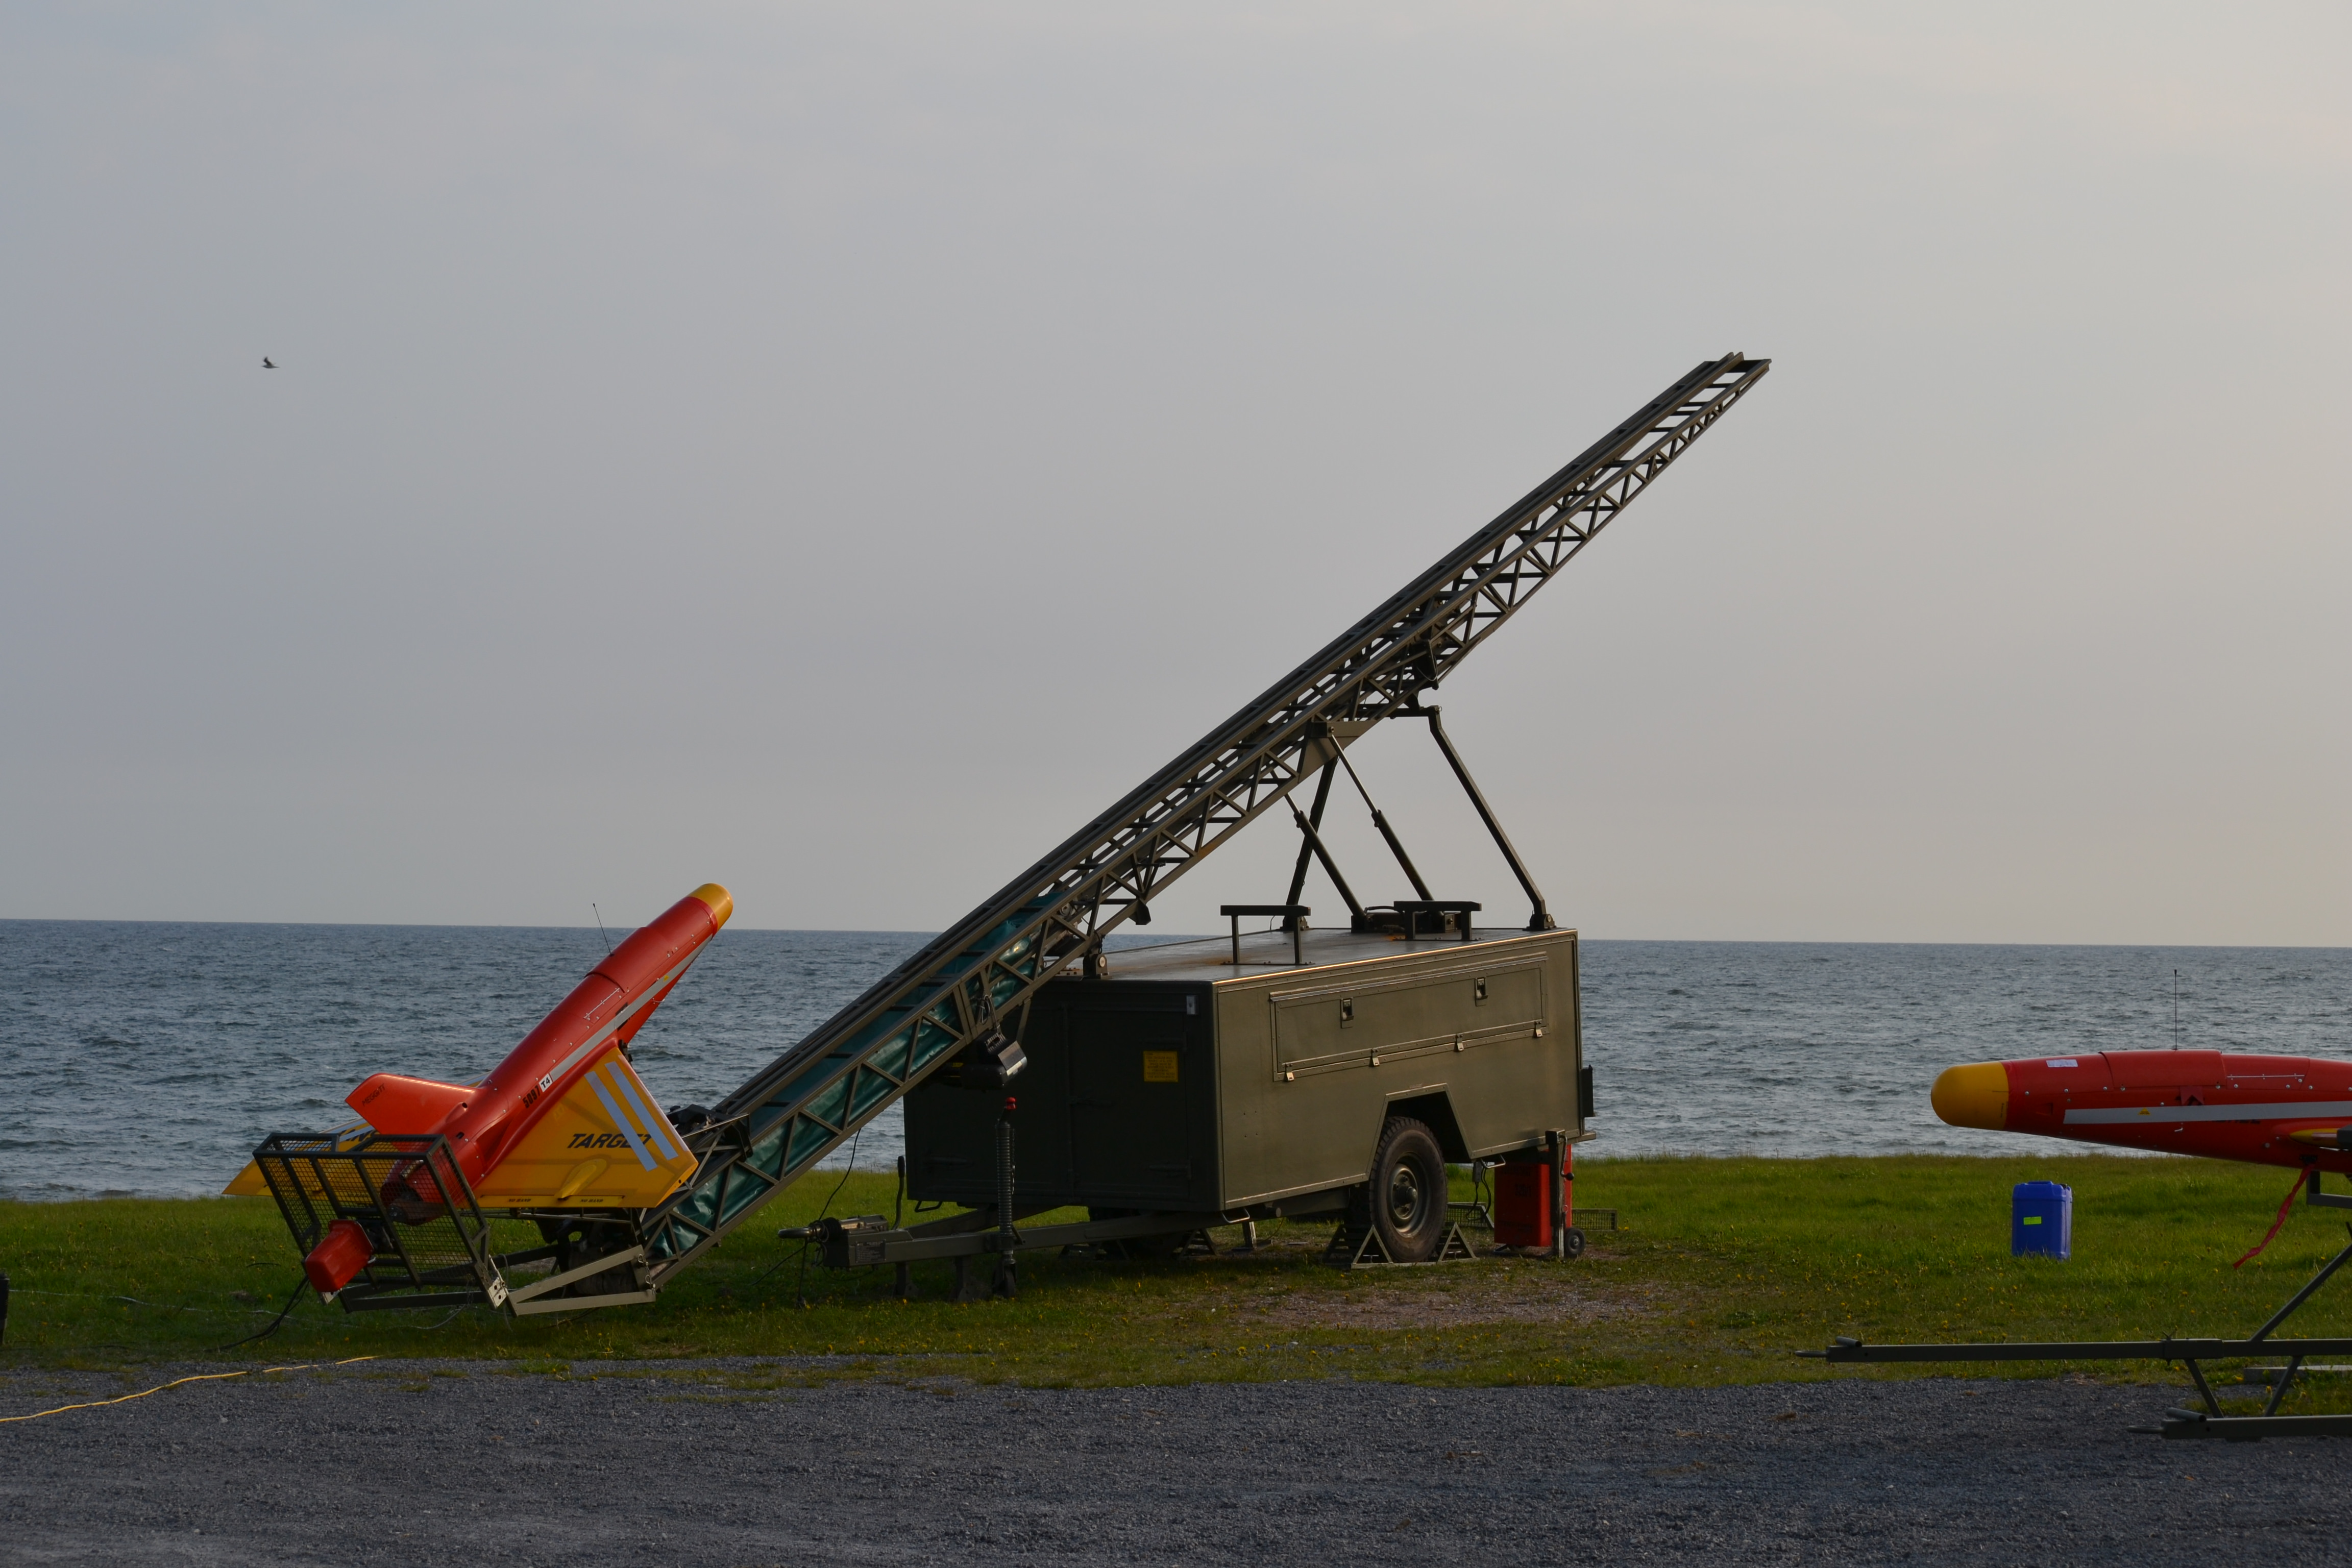
\includegraphics[width=1\linewidth]{kec-launcher.jpg}
		\caption[Short]{catapult launcher.}
		\label{fig:catapult}
	\end{figure}
	
	\begin{figure}[h]
		\centering
		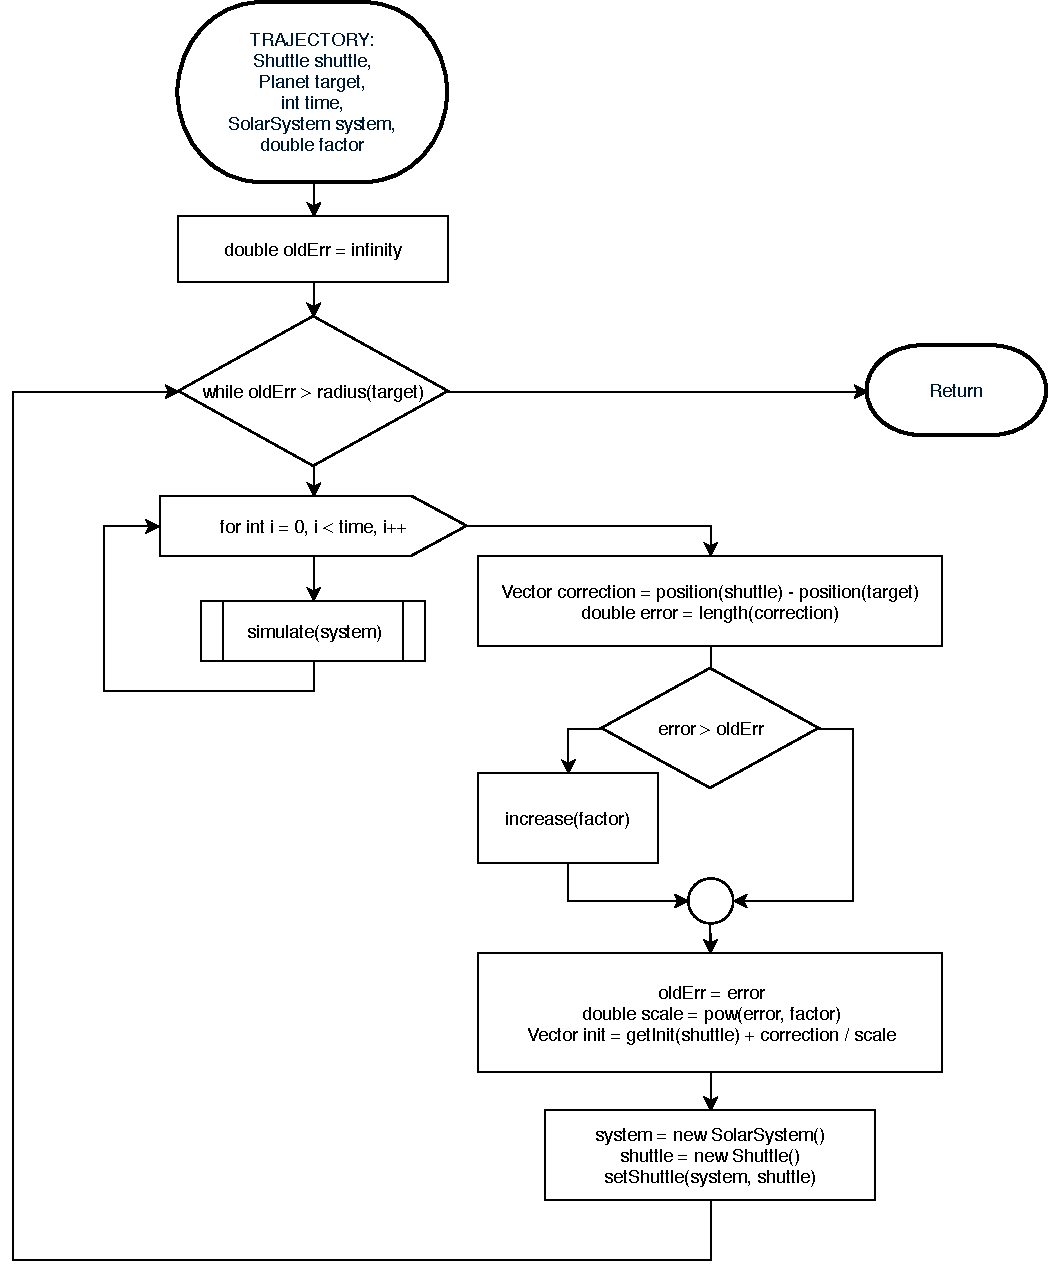
\includegraphics[width=1\linewidth]{trajectory}
		\caption[Short]{Algorithm to calculate the trajectory to reach a planet.}
		\label{fig:trajectory}
	\end{figure}
	
	\begin{figure}[h]
		\centering
		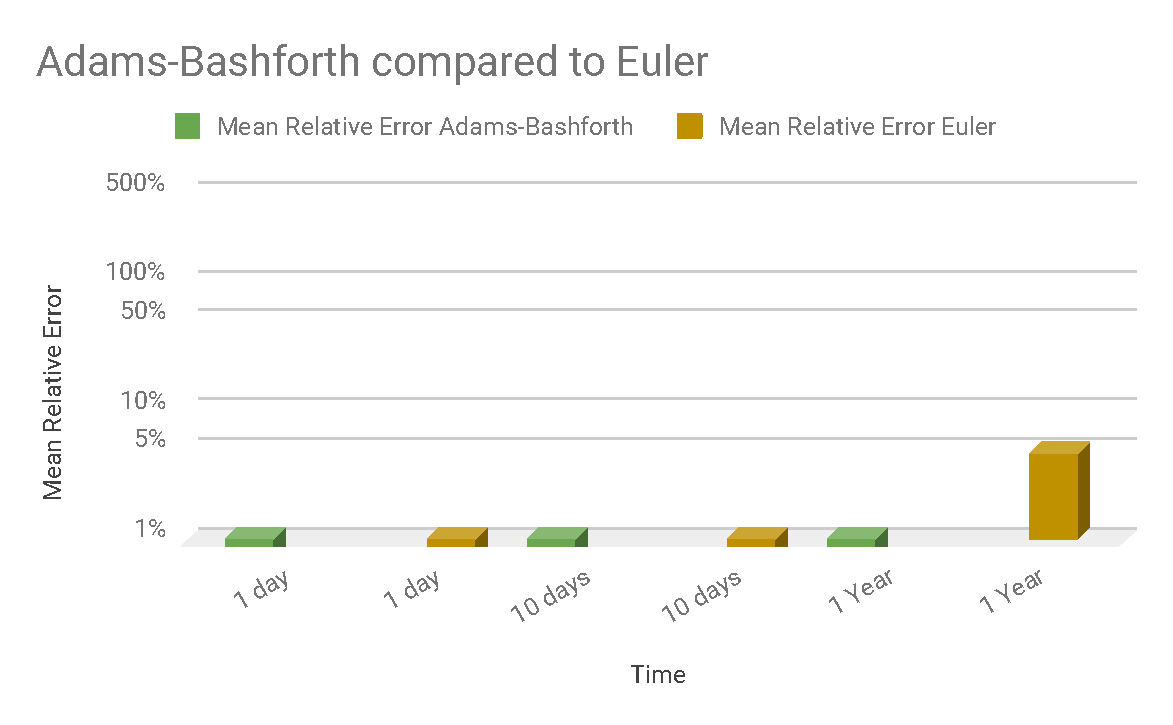
\includegraphics[width=1\linewidth]{Adams_Bashforth_compared_to_Euler.pdf}
		\caption[Short]{Adams-Bashforth's relative error compared to Euler's.}
		\label{fig:adams-bashforth}
	\end{figure}
	
	
	\begin{figure}[h]
		\centering
		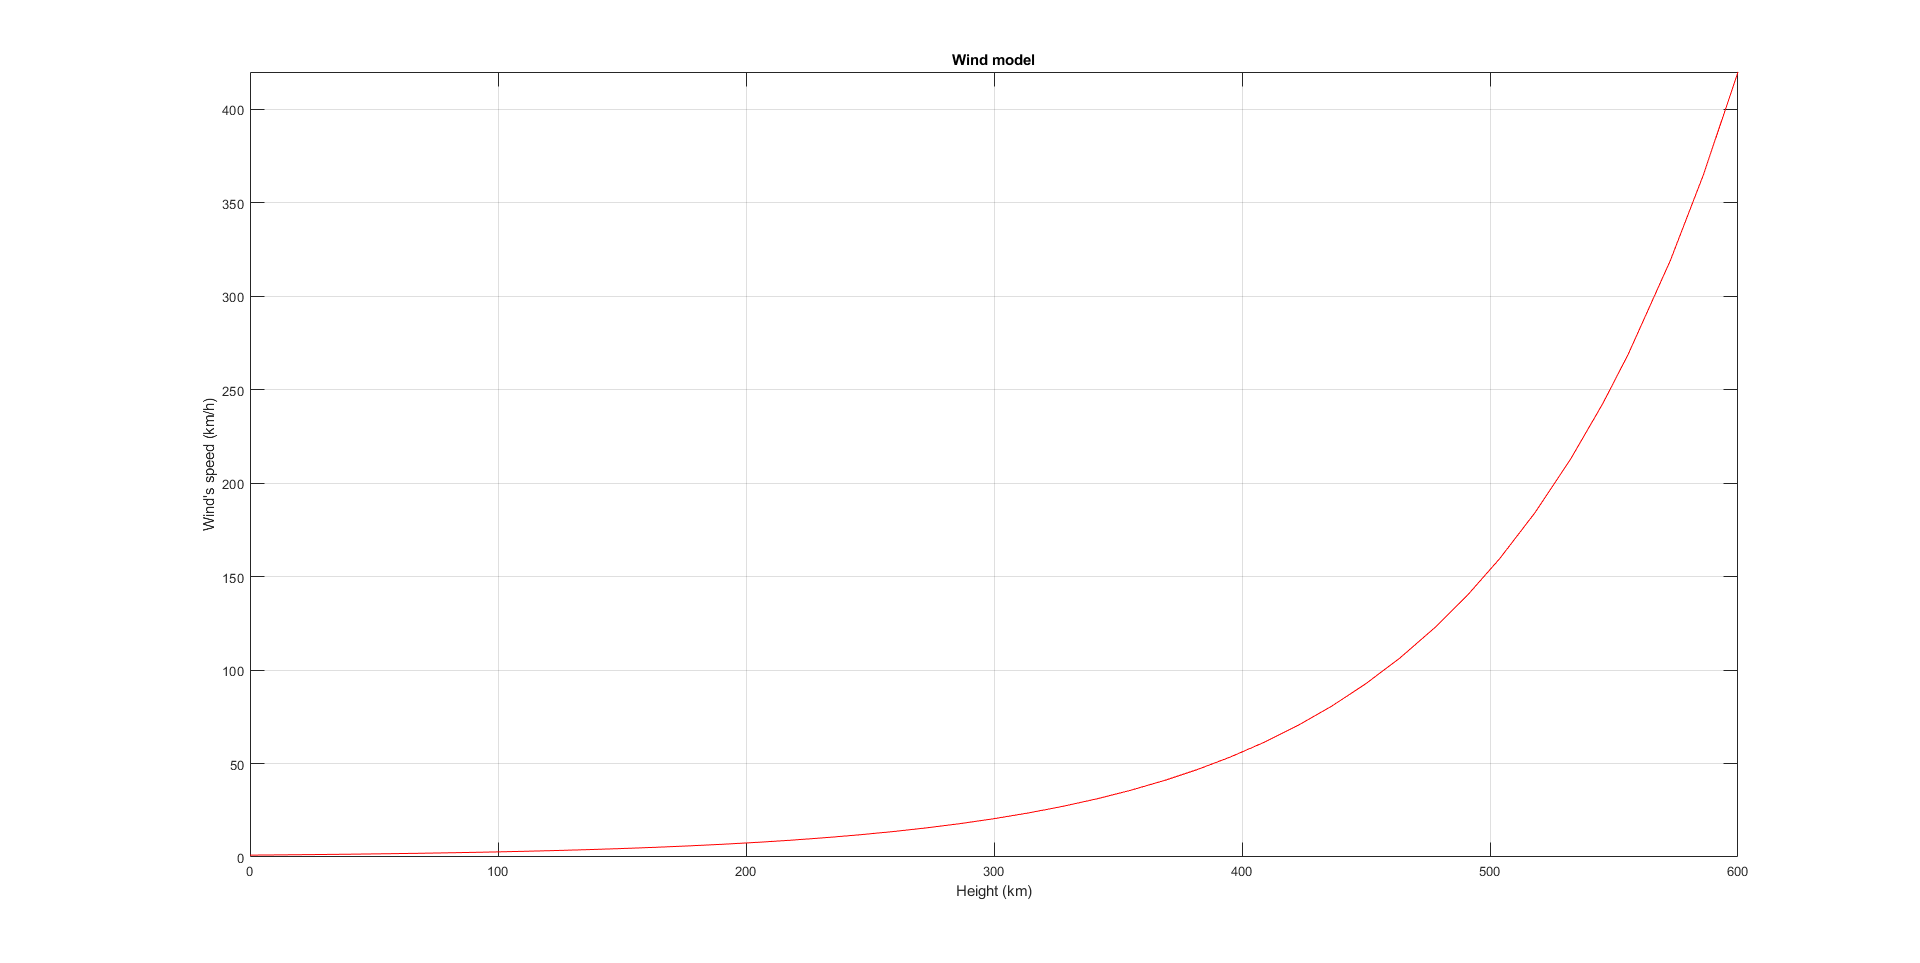
\includegraphics[width=1\linewidth]{wind_model.png}
		\caption[Short]{wind model.}
		\label{fig:wind}
	\end{figure}      
	
\end{document}
